%% Version 6.1, 1 September 2021
%
%%%%%%%%%%%%%%%%%%%%%%%%%%%%%%%%%%%%%%%%%%%%%%%%%%%%%%%%%%%%%%%%%%%%%%
% TemplateV6.1.tex --  LaTeX-based blank template for submissions to the 
% American Meteorological Society
%
%%%%%%%%%%%%%%%%%%%%%%%%%%%%%%%%%%%%%%%%%%%%%%%%%%%%%%%%%%%%%%%%%%%%%
% PREAMBLE
%%%%%%%%%%%%%%%%%%%%%%%%%%%%%%%%%%%%%%%%%%%%%%%%%%%%%%%%%%%%%%%%%%%%%

%% Start with one of the following:
% 1.5-SPACED VERSION FOR SUBMISSION TO THE AMS
\documentclass{ametsocV6.1}
\usepackage{slashbox}
\usepackage{longtable}
% TWO-COLUMN JOURNAL PAGE LAYOUT---FOR AUTHOR USE ONLY
% \documentclass[twocol]{ametsocV6.1}

%%%%%%%%%%%%%%%%%%%%%%%%%%%%%%%%

%%% To be entered by author:

%% May use \\ to break lines in title:

\title{Synergistic retrievals of ice in high clouds from elastic backscatter lidar, 
Ku-band radar and submillimeter wave radiometer observations}

%% Enter authors' names
% and affiliations as you see in the examples below.
%
%% Use \correspondingauthor{} and \thanks{} (\thanks command to be used for affiliations footnotes, 
%% such as current affiliation, additional affiliation, deceased, co-first authors, etc.)
%% immediately following the appropriate author.
%
%% Note that the \correspondingauthor{} command is NECESSARY.
%% The \thanks{} commands are OPTIONAL.
%
%% Enter affiliations within the \affiliation{} field. Use \aff{#} to indicate the affiliation letter at both the
%% affiliation and at each author's name. Use \\ to insert line breaks to place each affiliation on its own line.

%\authors{Author One,\aff{a}\correspondingauthor{Author One, email@email.com} 
%Author Two,\aff{a} 
%Author Three,\aff{b} 
%Author Four,\aff{a} 
%Author Five\thanks{Author Five's current affiliation: NCAR, Boulder, Colorado},\aff{c} 
%Author Six,\aff{c} 
%Author Seven,\aff{d}
% and Author Eight\aff{a,d}
%}
%
%\affiliation{\aff{a}{First Affiliation}\\
%\aff{b}{Second Affiliation}\\
%\aff{c}{Third Affiliation}\\
%\aff{d}{Fourth Affiliation}
%}

\authors{Mircea Grecu\aff{a,b}\correspondingauthor{Mircea Grecu, mircea.grecu-1@nasa.gov}
and John E. Yorks \aff{a}}
\affiliation{\aff{a}{NASA GSFC}\\
\aff{b}{Morgan State University}}

%%%%%%%%%%%%%%%%%%%%%%%%%%%%%%%%%%%%%%%%%%%%%%%%%%%%%%%%%%%%%%%%%%%%%
% ABSTRACT
%
% Enter your abstract here
% Abstracts should not exceed 250 words in length!
%
 
\abstract{ In this study, we investigate the synergy of elastic backscatter lidar, Ku-band radar, and sub-millimeter-wave radiometer measurements in the retrieval of ice from satellite observations. The synergy is analyzed through the generation of a large dataset of Ice Water Content (IWC) profiles and simulated lidar, radar and radiometer observations. The characteristics of the instruments e.g. frequencies, sensitivities, etc. are set based on the expected characteristics of instruments of the Atmosphere Observing System (AOS) mission. A hold-out validation methodology is used to assess the accuracy of the IWC profiles retrieved from various combinations of observations from the three instruments. Specifically, the IWC and associated observations are randomly divided into two datasets, one for training and the other for evaluation. The training dataset is used to train the retrieval algorithm, while the evaluation dataset is used to assess the retrieval performance. The dataset of IWC profiles is derived from CloudSat reflectivity and CALIOP lidar observations. The retrieval of the ice water content IWC profiles from the computed observations is achieved in two steps. In the first step, a class, out of 18 potential classes characterized by different vertical distribution of IWC, is estimated from the observations. The 18 classes are predetermined based on the k-Means clustering algorithm. In the second step, the IWC profile is estimated using an Ensemble Kalman Smoother (EKS) algorithm that uses the estimated class as a priori information.\\
The results of the study show that the synergy of lidar, radar, and radiometer observations is significant in the retrieval of the IWC profiles.  Nevertheless, it should be mentioned that this synergy was found under idealized conditions, and additional work might be required to materialize it in practice. The inclusion of the lidar backscatter observations in the retrieval process has a larger impact on the retrieval performance than the inclusion of the radar observations. As ice clouds have a significant impact on atmospheric radiative processes, this work is relevant to ongoing efforts to reduce uncertainties in climate analyses and projections.}



\begin{document}

%% Necessary!
\maketitle

%%%%%%%%%%%%%%%%%%%%%%%%%%%%%%%%%%%%%%%%%%%%%%%%%%%%%%%%%%%%%%%%%%%%%
% SIGNIFICANCE STATEMENT/CAPSULE SUMMARY
%%%%%%%%%%%%%%%%%%%%%%%%%%%%%%%%%%%%%%%%%%%%%%%%%%%%%%%%%%%%%%%%%%%%%
%
% If you are including an optional significance statement for a journal article or a required capsule summary for BAMS 
% (see www.ametsoc.org/ams/index.cfm/publications/authors/journal-and-bams-authors/formatting-and-manuscript-components for details), 
% please apply the necessary command as shown below:
%
% Significance Statement (all journals except BAMS)
%

%\statement
%This paper is significant.
%	 Enter significance statement here, no more than 120 words. See \url{www.ametsoc.org/index.cfm/ams/publications/author-information/significance-statements/} for details.
%
%% Capsule (BAMS only)
%%
%\capsule
%       Enter BAMS capsule here, no more than 30 words. See \url{www.ametsoc.org/index.cfm/ams/publications/author-information/formatting-and-manuscript-components/#capsule} for details.
%
%% * * If using twocol mode, you will need to use the commands "twocolsig" and "twocolcapsule" in place of "sig" and "capsule"
%%      to ensure that the text box correctly spans across both columns.
%

%%%%%%%%%%%%%%%%%%%%%%%%%%%%%%%%%%%%%%%%%%%%%%%%%%%%%%%%%%%%%%%%%%%%%
% MAIN BODY OF PAPER
%%%%%%%%%%%%%%%%%%%%%%%%%%%%%%%%%%%%%%%%%%%%%%%%%%%%%%%%%%%%%%%%%%%%%
%

%% In all cases, if there is only one entry of this type within
%% the higher level heading, use the star form: 
%%
\section{Introduction}
The future NASA Atmospheric Observing System (AOS) mission \citep{braun2022} is expected to feature new combinations of observations that may be used to quantify the amounts of ice in high clouds and characterize the microphysical properties of ice particles. In the AOS terminology, high clouds are convectively generated clouds \citep{braun2022}. They are the result of strong vertical mass transport accompanied by horizontal transport of hydrometeors in the upper troposphere.  As high clouds are of paramount importance in understanding the quantifying radiative processes, they constitute one of the AOS major objectives \citep{braun2022}. To achieve its objectives, AOS will rely on a combination of active and passive observations onboard multiple spacecrafts in two different orbits.  One of the orbits is expected to be polar, while the other is expected to be inclined, which would allow the study of atmospheric processes at sub-daily time scales, with an emphasis on deep convection, high clouds, and aerosols \citep{braun2022,yorks2022}. The AOS inclined observations will include backscatter from an elastic backscatter lidar \citep{weitkamp2006}, Ku-band radar reflectivity, and submillimeter wave radiometer brightness temperature measurements. 
While not necessarily optimal for cloud ice estimation, these measurements are complimentary and enable the synergistic characterization of ice clouds. That is, despite the fact that lidar observations attenuate quickly in thick ice clouds and the Ku-band radar will not be able to detect clouds characterized by an echo weaker than 8.0 dBZ (which is the expected sensitivity of the radar in the inclined orbit), the active observations are expected to provide context that may be incorporated into the radiometer retrievals. Herein, the term retrieval is defined as the process of estimating geophysical variables from remote sensing observations.
%, but, as customary in the scientific
%literature, estimates are occasionally referred to as retrievals as well.  
In this study, we investigate the impact of incorporating lidar and radar observations into the radiometer retrieval of ice clouds. Because the existing amount of coincident backscatter lidar, Ku-band radar, and submillimeter-wave  radiometer observations is rather insufficient to derive conclusive results, we employ accurate physical models to simulate lidar, radar and radiometer observations and use a hold-out validation methodology to characterize the retrieval accuracy. As estimates from passive instrument observations strongly depend on "a priori" information \citep{rodgers2000inverse}, for results to be relevant in real applications, it is necessary to base them on realistic vertical distributions of ice properties.  Such distributions may be derived from cloud-resolving-model (CRM) simulations \citep{pfreundschuh2020synergistic,liu2022assessing} or directly from observations.  In this study, we employ the latter approach, as CRMs may still be deficient in properly reproducing the vertical distribution of ice clouds and their associated microphysical properties.  Specifically, we use observations and products from the CloudSat (CS) mission (Stephens et al. 2002) to derive a database of ice microphysical properties and associated simulated lidar, radar, and radiometer observations.  To account for variability in the Particle Size Distributions (PSD) that may not be well represented in the 2C-ICE product, we use a simple but effective approach to perturb the PSD generalized intercepts from their nominal values. The resulting database is used to investigate the accuracy of estimated ice cloud properties from the simulated observations. Another major difference relative to previous studies is the unique combination of instruments investigated herein. It should be mentioned that although based on observations rather than CRM simulations, the approach used in this study is idealized in many respects. As a consequence, the results presented may not unbiasedly extrapolate to practice. Nonetheless, the results are expected to provide useful insights into the potential of the AOS inclined observations and good first step towards the development of an operational synergistic retrieval of ice clouds from AOS inclined observations. The article is organized as follows.  In Section 2, we describe the approach used to derive the ice properties and the associated simulated observations, the retrieval and the evaluation methodology.  In Section 3, we present the results of the evaluation methodology. We conclude in Section 4.

% \subsection*{subsection}
% text...
\section{Methodology}
As previously mentioned, we use CloudSat (CS) observations \citep{stephens2002} to derive the vertical distributions of ice properties needed in the investigation.  Although research quality CS cloud ice products exist, to maximize the physical consistency of the approach, we do not use them but derive ice amounts and associated properties directly from CS reflectivity observations.  This ensures the consistency between the particle distribution assumptions and the electromagnetic scattering properties used in the CS reflectivity processing and those used the simulation of the lidar, Ku-band radar and radiometer observations. Our CS-based ice product is optimized to be consistent with the synergistic Cloudsat and CALIPSO Ice Cloud Property Product (2C-ICE) of \cite{deng2015}.  When the CALIPSO lidar detects echo associated with clouds but the CS radar signal is below the noise level, we use the 2C-ICE product to extend our CS-based estimates. Specifically, we use the IWC estimates from the 2C-ICE product in conjunction with a Particle Size Distribution (PSD) generalized intercept \citep{testud2001} provided by statistical model described in the next section to characterize the ice PSDs of clouds with radar echo below the noise level of the CloudSat radar. Lidar, Ku-band radar, and submillimeter-wave radiometer observations are simulated from CS observations using accurate physical models and realistic assumptions consistent with the most recent knowledge in the field of ice cloud microphysics, and a non-parametric estimation methodology based on the k-Means clustering algorithm \cite{mackay2003information} is used to investigate the instrument synergy.  Details of the methodology are presented below.

\subsection{Assumptions and forward models}
To quantify the number of ice particles in an elementary atmospheric volume as a function of their size, we use normalized gamma functions \citep{bringi2003}.  The benefit of normalized gamma functions is that they encapsulate the variability of Ice Water Content (IWC) - reflectivity relationship into a single parameter, i.e. the normalized Particle Size Distribution (PSD) intercept \citep{testud2001,bringi2003}. The normalized PSD intercept is defined as $N_w=\frac {4^4} {\pi \rho_w} \frac {IWC} {D_m^4}$, where $IWC$ is the ice water content associated with the PSD, and $D_m$ is the mass weighted mean diameter.  Based on the work of \cite{testud2001}, \cite{ferreira2001} and \cite{delanoe2014} showed that the variability in IWC reflectivity (Z) relationships may be fully explained by variability in $N_w$, and that a formula of the type
\begin{equation}
IWC=N_w^{1-b}a_{norm} Z^b \label{eq:1}
\end{equation}
(where $a_{norm}$ and $b$ are constants) explains almost perfectly the relationships between IWC and Z calculated from observed PSDs.However, equation (\ref{eq:1}) is not  sufficient to derive accurate, unbiased estimates of ice water contents, because $N_w$ varies considerably in time and space. Nevertheless, multiple studies showed that it is beneficial to parameterize $N_w$ as a function  of various variables, such as temperature \citep{hogan2006retrieval, delanoe2008variational,deng2010tropical}, rather than using $N_w$ independent reflectivity ice relations.  In this study, we parameterize $N_w$ as a function of temperature based on the CloudSat 2C-ICE product \citep{deng2010tropical,deng2013evaluation}. A scatter-plot analysis of relationships between the 2C-ICE IWC and the associated reflectivity suggests that the multiplicative coefficient in a power low ice-reflectivity relationship is parameterized as a function of temperature (or equivalently, as a function of height relative to the freezing level) in the default 2C-ICE retrievals. The default multiplicative coefficient (the value the provides the IWC estimate prior to the ingestion of the lidar observations) may be simply estimated by regressing the 2C-ICE IWC on the associated CloudSat reflectivity as a function of $H$, defined as height relative the freezing level. Specifically, a regression of the type $ln(IWC)=ln(a)+b*ln(Z)$ is performed for each bin referenced relative to the zero degree bin is performed, and the variation of $ln(a)$ is parameterized as a function of the relative height.  The results are shown in Figure \ref{f2}. As apparent in the figure, and as expected, $a$ exhibits a strong variation with the relative height. Given that any deviation of the multiplicative coefficient in an IWC-Z relation from an average is equivalent to a deviation of the associated $N_w$ from its mean value \citep{ferreira2001,delanoe2014}, the variation of $a$ as a function of relative-height may be converted into an $N_w$ as a function of relative-height relationship.  We, therefore, use the data in Figure \ref{f2} to parameterize $N_w$ as a function of the relative height.  Specifically, given that $(1-b)ln(N_w)+ln(a_{norm})=ln(a)$ and $ln(a)=ln(a_0)+s*H$, with $a_0$ and $s$ the intercept and the slope of a regression for the data in Figure \ref{f2}, we can express $N_w$ as a function of the relative height, slope $s$, and parameters $a_0$ and $a_{norm}$.

\begin{figure}[t]
    \centering
    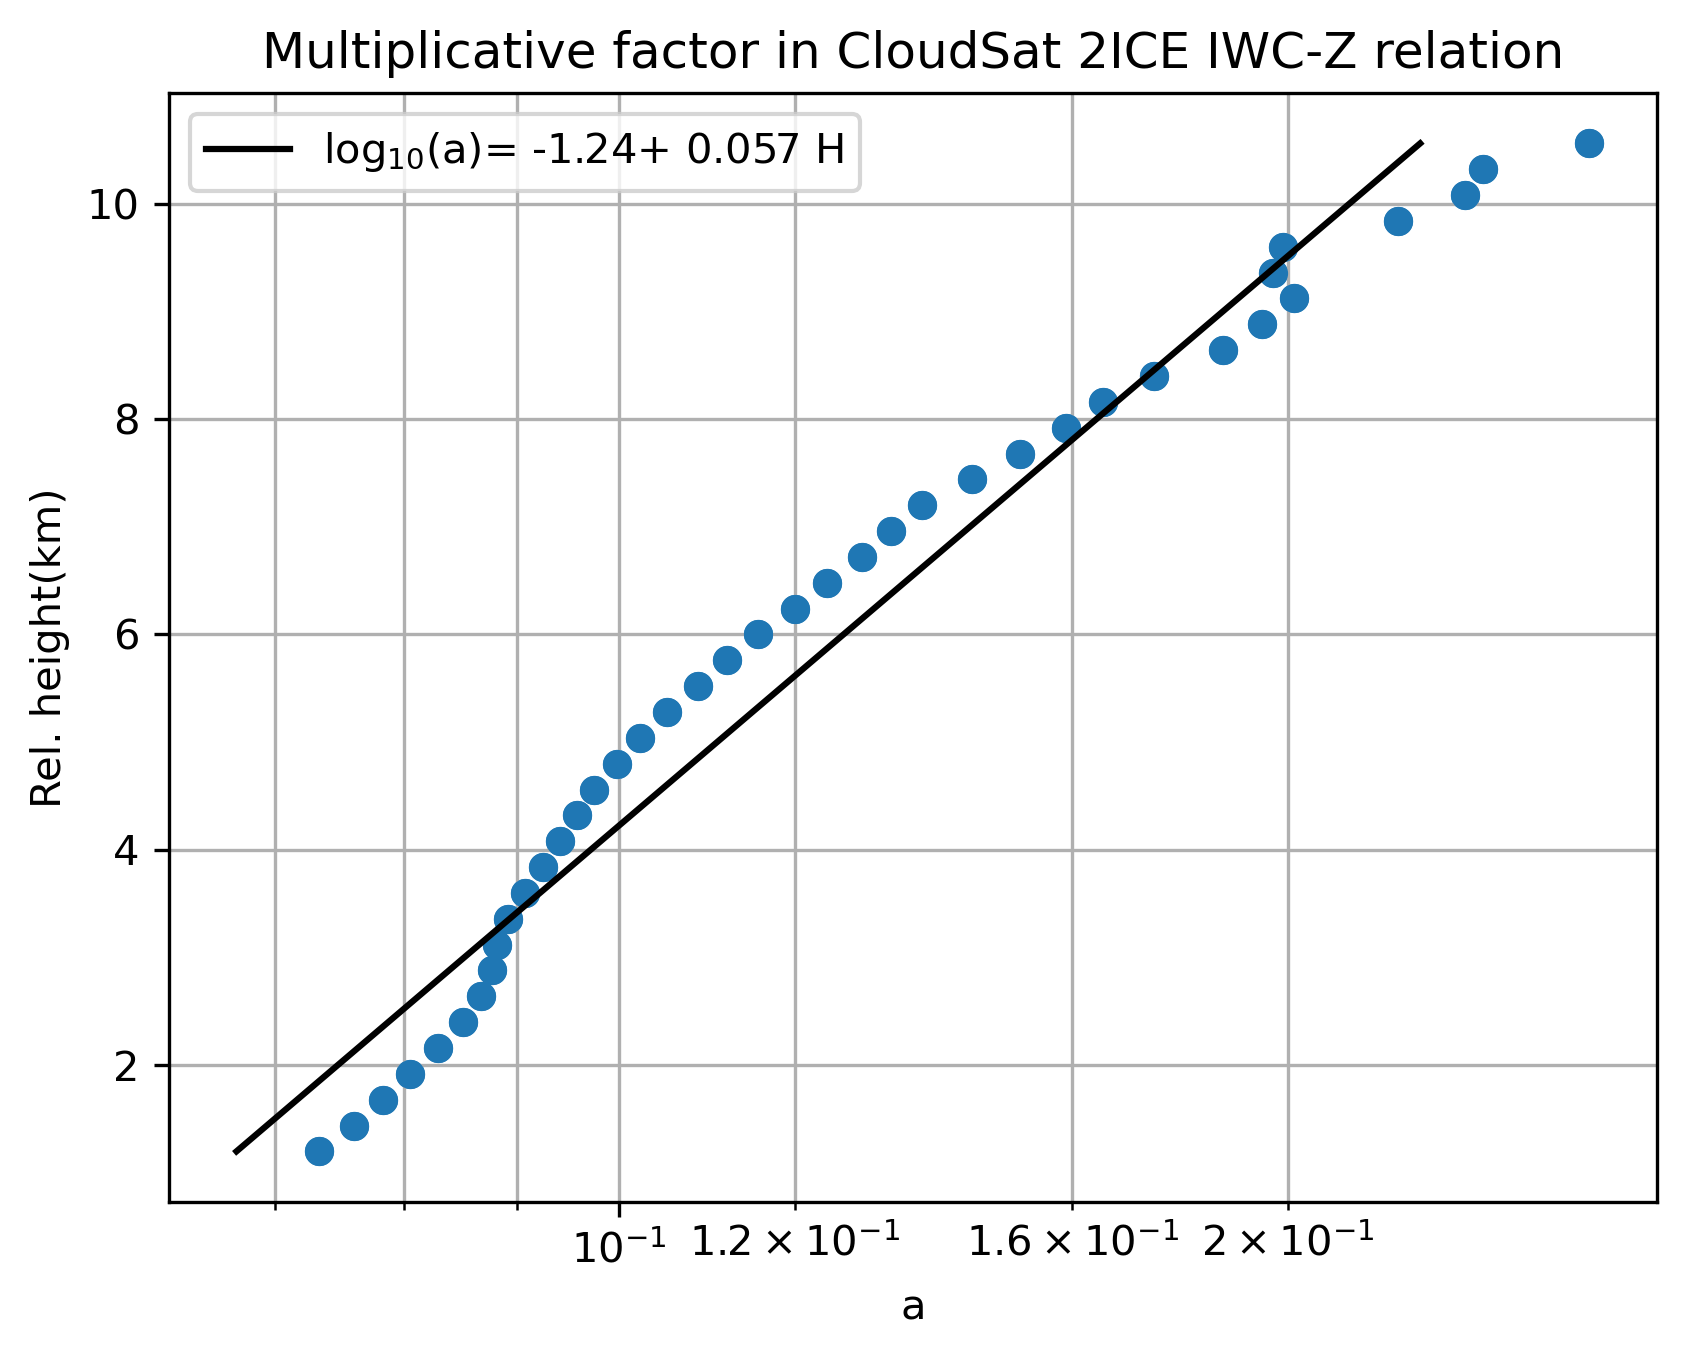
\includegraphics[width=0.75\textwidth,angle=0]{fig02.rev.png}\\
    \caption{Multiplicative factor in the 2ICE IWC-relation as a function of the height relative to the freezing level.}\label{f2}
\end{figure}

To investigate the variability in the vertical distribution of the 2C-ICE estimates and their consistency with our estimates, 
we cluster, based on similarity  (quantified through the evaluation of the Euclidian distance between profiles), a large set 2C-ICE profiles into 18 classes using a k-Means procedure. The mean IWC profiles associated with the 18 classes are shown in continuous lines in Figure \ref{f1}.  Our estimates, derived using PSD assumptions and electromagnetic scattering calculations that enable accurate and physically consistent simulations of radar observations at Ku-band and radiometer observations of submillimeter-wave frequencies are also shown in the figure. These estimates are based on the self-similarity Rayleigh-Gans approximation (SSRGA) of \cite{hogan2017ssrga}. Details regarding the estimation process are provided in the following paragraphs.  As apparent in Figure \ref{f1}, the CS and SSRGA estimates are in good agreement.  Some discrepancies due to differences between the SSRGA $N_w$ parameterization and the CS 2C-ICE "a priori assumptions" are also apparent, but they are not deemed critical in this study, whose objective is the investigation of synergistic lidar, Ku-band radar and submillimeter-wave radiometer retrievals, because the outcome is not likely to be sensitive to such details. Also apparent in Figure \ref{f1} is the fact that there is significant variability in the vertical distribution of the 2C-ICE IWC estimates, which makes the estimation of IWC profiles from passive-only observations challenging.  

\begin{figure}[t]
    \centering
    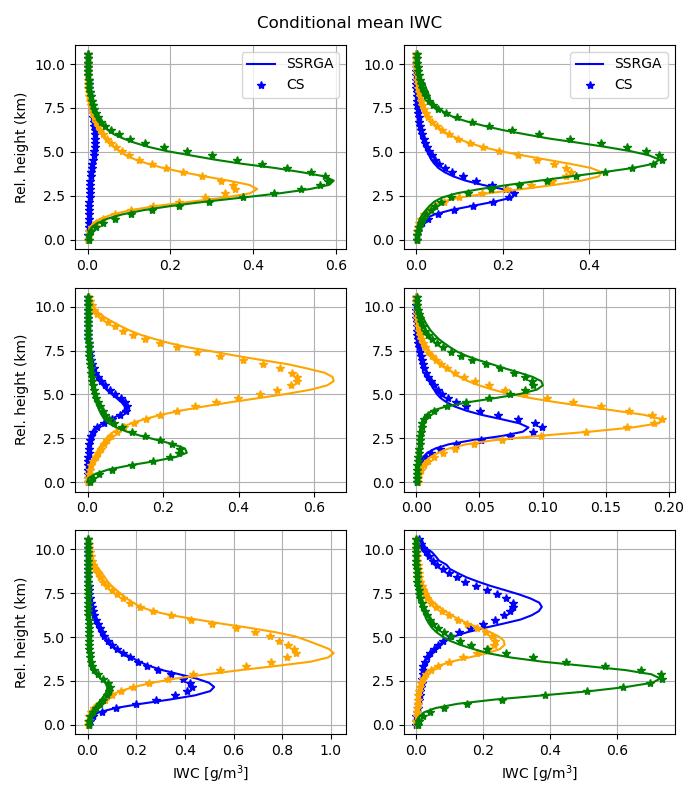
\includegraphics[width=0.75\textwidth,angle=0]{fig01.png}\\
    \caption{Mean CS IWC profiles for 18 classes derived using the k-Means clustering algorithm. For a 
    compressed but intelligible representation, three classes are shown in different colors in each panel.
    The associated 
    mean profiles derived from CS reflectivity observations using the SSRGA scattering calculations 
    and $N_w$ parameterization developed in this study are shown using symbol *. The vertical coordinate 
    is defined relative to the freezing level.}\label{f1}
\end{figure}

For the determination of reference $a_{norm}$ and $b$ values to be used with Equation (\ref{eq:1}), we assume that PSDs are normalized gamma  distributions with $N_w=0.08cm^{-4}$ and $\mu=2$ and calculate 
\begin{equation}
 Z=\frac {\lambda ^4} {\pi ^5 |K_w|^2} \int_0^{\infty} N(D,D_m) \sigma _b(D) dD
\end{equation}
where $\lambda$ is the radar frequency, $|K_w|$ is the dielectric factor of water, $N(D,D_m) dD$ is the number of ice particles of diameter with D and D+dD per unit volume, $D_m$ is the mass weighted mean diameter of the distribution, and $\sigma _b(D)$ is the backscattering cross-section of ice particle of diameter $D$. The mass weighted mean diameter is equidistantly sampled to span the entire range of IWC values in the CS 2C-ICE dataset. The assumed mass-size relation is that of \cite{brown1995improved} because it works well with the SSRGA scattering calculations \citep{heymsfield2022impacts}.  The open source software scatter-1.1 of \citep{scatter-1.1} is used to provide the actual scattering properties. To improve the representation of microphysical variability in the study, we do not assume the values of $N_w$ given by the 2C-ICE based parametrization described above as the true values. Instead, we perturb them by multiplication with a log-normally distributed random variable with 0.0 mean a standard deviation of 0.5.  The perturbations are vertically correlated. Specifically, normal random variables with zero mean and a standard deviation of 1.0 are generated and then passed through a Gaussian smoothing filter \citep{nixon2019} with a size of two radar bins. The perturbation vector is then rescaled to have a standard deviation of 0.5.  The perturbations are then exponentiated and multiplied with the 2C-ICE based $N_w$ values to produce the final $N_w$ values.  The filter size and noise magnitude are chosen to roughly mimic the observed variability in $N_w$ derived from in situ observations of PSDs, such as those described in \cite{heymsfield2022impacts}. In addition, we are adding a random noise of 0.0 mean and 0.5 dB standard deviation to the calculated reflectivity values, which is consistent with the expected performance of a space-borne Ku-band radar system \citep{takahashi2008}.  Nevertheless, it should be noted that the uncertainties in the reflectivity calculations are likely to be even larger, given that the SSRGA theory, although quite accurate, cannot possibly capture the entire range of uncertainties in the scattering properties of ice particles. Specifically, the SSRGA calculations were carried out assuming ice particles consisting of aggregates of bullet rosettes, columnar crystals, and plates.

Moreover, the SSRGA theory was developed for millimeter and submillimeter-wave calculations and may not be applicable at lidar's wavelength. Therefore, lidar observations are computed using the Mie solution included in the scatter-1.1 package for a backscatter lidar, given that such a lidar is expected to be flown with a Ku-band radar and microwave radiometer as part of the NASA Earth System Observatory (ESO) Atmosphere Observing System (AOS) in an inclined and/or polar orbit \citep{yorks2022}.While uncertainties in the lidar forward model are rather complex and difficult to quantify, uncertainties in the lidar observations may be accounted for to some extent by including a multiplicative random noise factor in the calculated lidar backscatter values. Specifically, the calculated lidar backscatter values are multiplied with a log-normally distributed random variable with 0.0 mean and a standard deviation of 0.1. This results in uncertainties of about 10\% in the lidar backscatter values, conservative compared to the expected performance of the AOS lidars at 532 nm but consistent the performance of Cloud-Aerosol Transport System (CATS) lidar system at 1064 nm reported in \citep{pauly2019}. While the AOS lidars will have expected backscatter accuracies of 2-5\%, the lidar simulations in this paper are rather idealized in that they do not include random errors due to daytime solar background noise or systematic errors such as calibration accuracy or lidar ratio assumptions. More advanced models of the observation errors exist \citep{liu2006}, but are not considered here. There are three main reasons this approach was taken: (1) it is important to understand the limitations of combining these three datasets before factoring in individual sensor limitations, (2) while more accurate calculations based on more realistic ice particle shapes exist, they are rather incomplete and not readily available, and (3) Wagner and Delene (2022) compared lidar backscatter observations with backscatter calculations based on coincident PSD observations and the Mie solution and found good agreement, which suggests that electromagnetic properties derived from Mie calculations are adequate for practical applications. The lidar molecular backscatter and extinction are calculated using the lidar module of the CFMIP Observation Simulator Package (COSP; Bodas-Salcedo et al. (2011)). COSP simulates the lidar total attenuated backscatter signal and scattering ratios at 532 nm for scenes with and without clouds. COSP also assumes cloud particles are spherical so that the backscattering phase function is estimated based on the effective radius (Mie theory). Despite this assumption, the COSP simulations agree well with CALIOP observations. To account for multiple-scattering in the lidar observations, we are using the multiscatter-1.2.11 model \citep{multiscatter-1.2.11} of \cite{hogan2008lidar_ms}. 

Shown in Figure 3 are the distributions of simulated Ku-band radar reflectivity and lidar backscatter as function of height above the freezing level. As apparent in the figure, the IWCs associated with detectable Ku-band reflectivity signal are likely to occur near mostly around 3.0 km above the freezing level, while the lidar backscatter distribution exhibits a peak at around 6.0-7.0 km above the freezing level, which is consistent with the fact the lidar observations are strongly attenuated in the bottom part of the cloud.  It should be noted that, consistently with the objective of this study, only CS reflectivity profiles with no echo at or below the freezing level were selected and used in the calculation of Ku-band reflectivity distributions shown in Figure \ref{f3}. The vertical resolutions of the radar and lidar observations are the same, i.e. 240 m, and the same as the resolution of the CS observations upon which they are based. In reality, the radar and lidar observations are likely to have different vertical resolutions and footprint sizes, which would need to be accounted for in a more realistic study.  It should be noted though that the AOS radars and radiometers are expected to achieveNyquist sampling, which enables resolution enhancement \citep{early2001image}.  Nevertheless, differences in the vertical resolutions of the radar and lidar observations and differences in the footprint sizes may deteriorate the performance of the retrieval algorithm.

\begin{figure}[t]
    \centering
    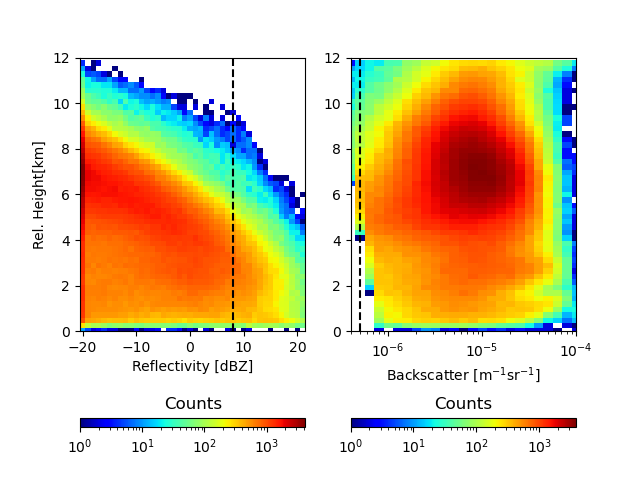
\includegraphics[width=0.75\textwidth,angle=0]{fig03.rev.png}\\
    \caption{Simulated distributions of Ku-band radar reflectivity (left) and lidar backscatter (right)
    as function of height above 
    the freezing level. Vertical lines indicated the assumed instrument sensitivities (8dBZ for the 
    radar and 5e-7 m$^{-1}$ sr$^{-1}$ for the lidar, respectively.) }\label{f3}
\end{figure}

The radiometer observations are calculated using a one-dimensional efficient, but accurate, radiative transfer  solver based on Eddington's approximation \citep{kummerow1993edd}. The Eddington's approximation has been found to work well in cloud and precipitation retrieval application despite its simplicity relative to more general (but also computationally intensive) approaches such as Monte Carlo radiative transfer solvers \citep{liu1996three} It should be noted tough that the phase functions of ice particles tend to be highly asymmetric at sub-millimeter wave frequencies. For radiative transfer solutions based on the Eddington's approximation to be accurate, it is necessary that the delta-scaling approach \citep{joseph1976delta} be employed. The delta-scaling approach transforms the initial radiative transfer equation into an equivalent one characterized by a less asymmetric scattering function and more extinction, which makes the solution Eddington approximation more stable and accurate. The absorption due to water vapor and other gases is quantified using the Rosenkranz model \citep{rosenkranz1998}.  The water vapor, temperature, and pressure distributions are derived based on a WRF simulation of summer convection over the United States.  Specifically, the water vapor, temperature, and pressure profiles associated with times and areas where the model produces anvils are selected and clustered into 40 classes using the k-Means approach.  The mean extinction profiles at the radiometer frequencies are calculated for every class and used in process of calculating the brightness temperatures from the estimated ice profiles using a simple Monte Carlo procedure.  That is, given a retrieved ice profile and its scattering property, an anvil class and its associated absorption, temperature, and pressure profiles are randomly selected and attached to the ice scattering properties. To make the procedure physically meaningful, temperature rather than height is used in the ice scattering-gas absorption collocation process.  The surface emissivities are randomly chosen between 0.8 and 1.0 and assumed constant for all radiometer frequencies.  Brightness temperatures are calculated at 
%89-, 183.31 ± 1.1, and 325.15 ± 1.5 GHz,
all frequencies of the 10 channels of the SAPHIR-NG radiometer envisioned to be deployed in the AOS mission \citep{brogniez2022time}.  One of the frequencies is 89-GHz, while the others are centered on the 183.31, and 325.15 GHz water vapor absorption lines. Details regarding the radiometer and the active instruments are provided in Table \ref{t_sensors}.  Errors in the radiometer observations are modeled assuming a Noise-Equivalent-Delta-T (NEDT) of 1K, which is a readily achievable level for modern satellite radiometers \citep{draper2015}.

The processing steps used to process the CS reflectivity observations and calculate the lidar, Ku-band and submillimeter-wave radiometer observations may be summarized as follows:
\begin{enumerate}
\item Derivation of physically consistent radar and radiometer lookup tables to relate basic radar and radiometer properties (e.g. reflectivity, attenuation, extinction, scattering-albedo, etc.) to PSD parameters such as $IWC$ and $D_m$. The tables are derived for a single of $N_w$, but are usable with any value of 
$N_w$ using the "normalization" operations described in \citep{grecu2011}.
\item Derivation of $N_w$-relative height parameterization using the 2C-ICE product.
\item Estimation of IWC and related PSD parameters from CS W-band radar observations, using the tables constructed Step 1, and $N_w$ profiles derived through parameterization obtained in Step 2 and perturbed using the random model described above. Specifically, given $N_w$ and the associated $Z$ at W-band, we estimate $IWC/N_w$ as a function of $Z/N_w$ using the normalized tables and then derive $IWC$ from $IWC/N_w$ and $N_w$.  A simple forward attenuation correction \citep{meneghini1978} is applied to the W-band reflectivity observations prior to the estimation of $IWC$.  Attenuation due to water vapor and other gases is calculated using the Rosenkranz model \citep{rosenkranz1998} assuming the same temperature, pressure and temperature profiles used in the radiometer simulations.

\item Calculation of lidar, Ku-band radar and radiometer observations from the estimates derived in Step 3 and the tables obtained in Step 1, and extended with non-zero 2C-ICE estimates for the radar bins characterized by no echo
above the noise level.
\end{enumerate}

\begin{table}
    \caption{Assumed instrument characteristics.}\label{t_sensors}
    \begin{center}
    \begin{tabular}{llll}

    Instrument & Frequency/Wavelength & Noise Assumptions& Sensitivity \\
    \hline
    Lidar & 532 nm & LogNormal(0,0.1) & 5e-7 m$^{-1}$sr$^{-1}$ \\
    \hline
    Radar & 13.8 GHz & 0.5dB & 8 dBZ \\
    \hline
    Radiometer & 89 GHz & 1.0 K & N/A \\
    & 183.31+/-0.2 GHz & 1.0 K & N/A \\
    & 183.31+/-1.1 GHz & 1.0 K & N/A \\
    & 183.31+/-2.8 GHz & 1.0 K & N/A \\
    & 183.31+/-4.2 GHz & 1.0 K & N/A \\
    & 183.31+/-6.8 GHz & 1.0 K & N/A \\
    & 183.31+/-11 GHz & 1.0 K & N/A \\
    & 325.15+/-1.5 GHz & 1.0 K & N/A \\
    & 325.15+/-3.5 GHz & 1.0 K & N/A \\
    & 325.15+/-9.5 GHz & 1.0 K & N/A \\
   \hline \\
    
    \end{tabular}
\end{center}
\end{table}


The application of these steps produces a large dataset of approximately 800,000 cloud ice profiles and associated lidar, radar and radiometer observations that may be used to investigate the synergy of the three sensors. Details are provided in the next section.

\subsection{Estimation and evaluation}
Given that the lidar observations may attenuate quickly in thick clouds, while the Ku-band radar will not detect clouds with an echo weaker than 8.0 dBZ, the radiometer is the instrument likely to provide by itself the most complete information about the total amount of ice in its observing volume.  However, the vertical distribution of ice is difficult to quantify from radiometer-only observations, because significantly different ice vertical distributions may lead to very similar radiometer observations.  This makes radiometer-only retrievals highly dependent on the "a priori" information on the distribution of ice clouds in the atmosphere. As previously mentioned, this is the reason why CS-based IWC retrievals were preferred to CRM simulations, as retrievals are expected to result in more natural and less biased distributions. 

For retrievals, we employ a two-step estimation methodology similar to that of \cite{grecu2018}.  In the first step, we 
estimate an IWC class, out of the 18 classes of shown in Figure \ref{f1}, to which the estimated IWC profile is most likely to belong. The class estimation procedure is trained using the synthetic observations. In the second step, we estimate the IWC profile, using a class specific ensemble Kalman Smoother (EKS) methodology similar to that of \cite{grecu2018}. The EKS algorithm updates the estimated IWC relative to the mean IWC of the class to which the profile belongs. The differences between the actual active and passive observations and their mean class values are used in the update. The second step of this procedure is formally identical to the one used in \cite{grecu2018}, but the first step is different. In \cite{grecu2018}, the first step was based on a simple distance-based evaluation. That strategy is likely to be suboptimal in this study, because the joint distribution of IWC profiles and associated observations are significantly more complex. We, therefore, use a more complex classification methodology based on the TensorFlow library \citep{tensorflow2016}. The class estimation model is defined as a
TensorFlow Model with two dense layers of 30 neurons each, followed by a softmax layer \citep{deepL2016}. The activation function used in the dense layer is Rectified Linear Unit (ReLU) \citep{nair2010}. The class estimation model is trained using the 70\% of the simulated observations and the corresponding IWC profiles, while the remaining 30\% of the data being used for evaluation. The EKS update is based on formula%The training is done using the Adam
\begin{equation}
    \mathbf{X}=\mathbf{\bar{X}_i}+\mathbf{Cov(X_i,Y_i)}\mathbf{Cov(Y_i,Y_i)}^{-1}(\mathbf{Y}-\mathbf{\bar{Y}_i}) \label{eq:enks}
\end{equation}
where $\mathbf{X}$ is the state variable describing the IWC profile, $\mathbf{Y}$ is the vector containing the actual observations, $\mathbf{X_i}$ is the set of state variables for profiles in class $i$, and $\mathbf{Y_i}$ is the set of observations associated with profiles in class $i$.  Variables $\mathbf{\bar{X}_i}$ and $\mathbf{\bar{Y}_i}$ are the mean values of the state variables and observations in class $i$, respectively. The covariance matrices between  $\mathbf{X_i}$ and $\mathbf{Y_i}$ are denoted by $\mathbf{Cov(X_i,Y_i)}$. In step 1, the class is estimated using the TensorFlow model, while in step 2, the IWC profile is estimated using the EKS algorithm summarized in Equation \ref{eq:enks}.

As already mentioned, a hold-out validation methodology is used for evaluation, with 70\% of the data used for training and the remaining 30\% of the data used for validation.  The partition of the data into training and evaluation subsets is done randomly.  In a more general cross-validation methodology, the partition, training and evaluation steps are repeated several times.  However, given the fact that differences in the relationships between the ice property and their associated simulated observations are functions of the meteorological context, and that all regimes are well-sampled in both the training and testing subsets (e.g. out of every 10 pixels in a scene, about seven end up in the training dataset, while the others in the testing dataset), the repetition of the partition, training, and evaluation steps multiple times is not necessary. Therefore, in our evaluation, we partition the data into training and evaluation only once and perform all the evaluation for a single partition. The evaluation criteria include the correlation coefficient, the bias, and visual inspections of graphical representations of the estimated properties relative to their references.
%vs

\section{Results}
\subsection{Radiometer-only retrievals}
As previously mentioned, submillimeter-wave radiometers are likely to provide by themselves more complete information about the total amount of ice in their observing volumes than lidars or Ku-band radars with limited sensitivity. However, radiometers observations are an integrated measure of radiative processes in clouds that provide little information about the vertical distribution of ice. From this perspective, an evaluation in terms of the ice water path (IWP) defined as the vertical integral of the IWC, i.e. $IWP=\int_0^{Z_{top}}IWC(z)dz$ is insightful.  Shown in Figure \ref{f4} is the distribution of IWP estimated from radiometer-only observations as a function of its true value. As apparent in the figure, there is good correlation between the retrieved and the true IWP values. The numerical value of the correlation coefficient is 0.92, and there is no-overall bias. That is, the mean values of retrieved IWP and true IWP values are equal. However, conditional biases are apparent, with overestimation of IWP for values smaller than 100 g/$m^2$ and some underestimation for values larger than 1000 g/$m^2$.  The biases at the low end of the IWP range are not surprising, given that the impact caused by ice scattering on the total radiometric signal is small for low values of IWP and hard to distinguish from other sources of variability in radiometer observations. Saturation effects are most likely responsible for underestimation at the high end.  It should be noted that in this evaluation, only atmospheric profiles that exhibit ice detectable by the CS radar or CALIOP lidar are used. Therefore, a radiometer-only estimation procedure derived from this training dataset is likely to result in significant overestimation if not used in conjunction with a discrimination procedure. However, such procedure is not critical in this study, as, in a synergistic application, the lidar observations may be used to discriminate between clear skies and ice clouds.
\begin{figure}[t]
    \centering
    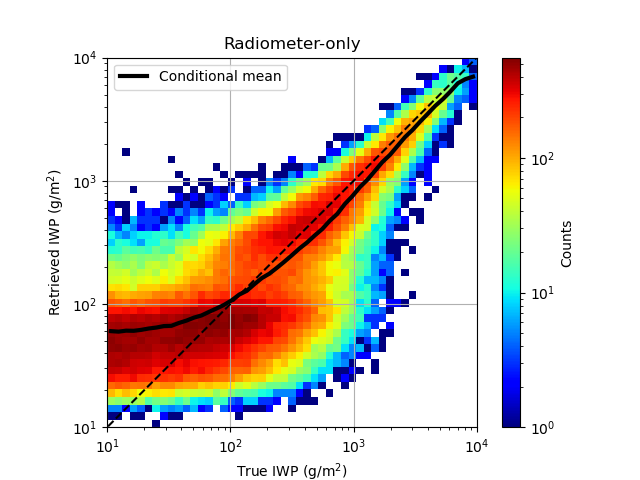
\includegraphics[width=0.75\textwidth,angle=0]{fig04.rev.png}\\
    \caption{Frequency plot of estimated IWP derived radiometer-observations as a function of the 
    true IWP used in observations synthesis.}\label{f4}
\end{figure}
However, although the radiometer-only estimation procedure is able to estimate the integrated amount of ice in clouds fairly
well, its ability to characterize the vertical distribution of ice in clouds is limited.  Figure \ref{f5} shows the conditional vertical distributions of the estimated and true IWC for the 18 classes described in Section 2a and shown in Figure \ref{f1}. As apparent in the figure, there are significant differences between the estimated and true IWC profiles. 
\begin{figure}[t]
    \centering
    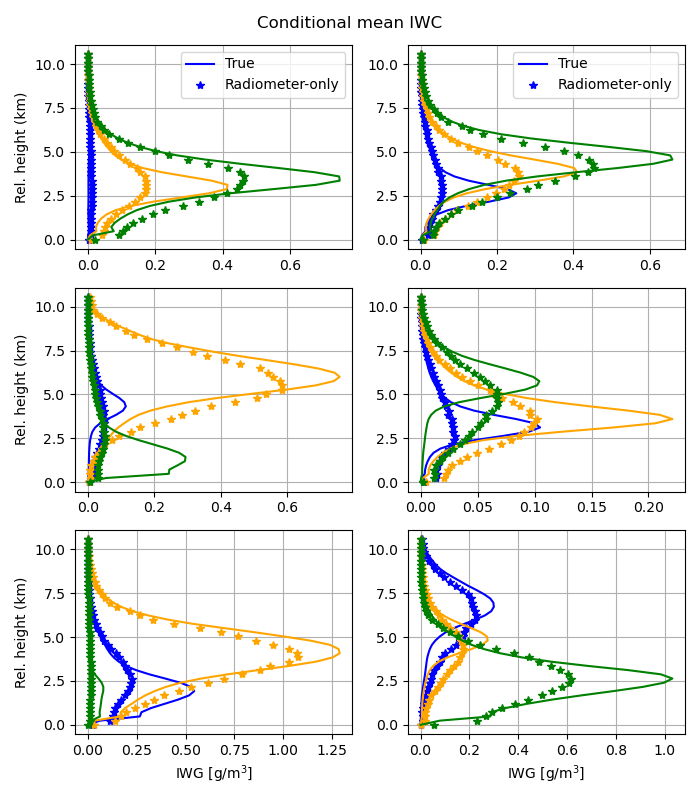
\includegraphics[width=0.75\textwidth,angle=0]{fig05.rev.png}\\
    \caption{True and radiometer-only retrieved conditional mean IWC for the 18 classes described in 
    Figure \ref{f1}.}\label{f5}
\end{figure}

Further insight into the radiometer-only estimation performance may be derived by defining the ice profile gravity center (GC) as $z_{GC}=\frac {\int_0^{Z_{top}}zIWC(z)dz} {\int_0^{Z_{top}}IWC(z)dz}$, where $z$ is the distance relative to the freezing level, the $Z_{top}$ is the distance from the top of the atmosphere to the freezing level. Shown in Figure \ref{f6} is the frequency of IWC gravity center estimated from radiometer-only observations as a function of its true value.  It may be observed in the figure that while the true IWC gravity center exhibits quite a broad distribution, the one retrieved from the radiometer-only observations exhibits a multimodal narrow distribution. Moreover, there correlation between the retrieved and the true IWC gravity center is rather low.  This is another indication that, while the total amount of ice may be reasonably estimated from radiometer-only observations, its vertical distribution can not be accurately determined from radiometer-only observations.

\begin{figure}[t]
    \centering
    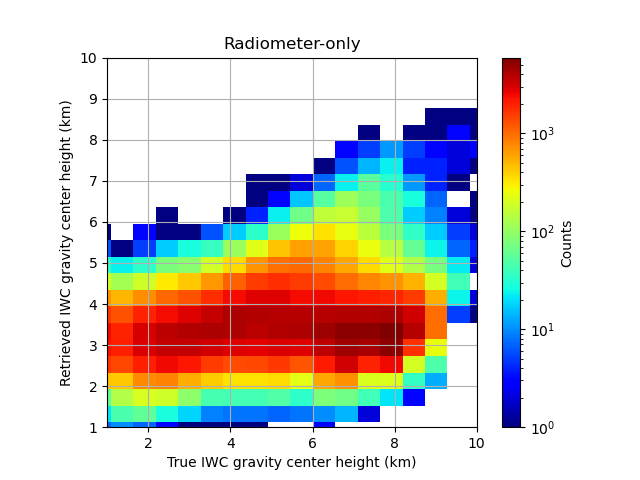
\includegraphics[width=0.75\textwidth,angle=0]{fig06.rev.png}\\
    \caption{Same as in Figure \ref{f4}, but for the IWC gravity center.}\label{f6}
\end{figure}

\subsection{Active instrument retrievals}

Although retrievals from the lidar-only or radar-only observations are not expected to be as accurate as those from radiometer-only observations, the lidar observations being subject to severe attenuation while the radar observations being limited by sensitivity, they are nevertheless insightful. This is because quantifying the limitations of retrievals from active instruments may be used to better assess  the benefits of synergistic retrievals.  Shown in the left column of Figure \ref{f7} are the distributions of IWP estimated from lidar-only and radar-only observations as a function of their true values. As apparent in the figure, and as expected, the lidar-only retrievals tend to be accurate for IWP values smaller than 50 g/m$^2$, while the radar-only retrievals tend to be reliable only for large IWP values on the order of hundreds of g/m$^2$.  Not that the radar-only retrievals exhibit a bimodal distributions,with a broad distribution of real IWP values associated with a single retrieved IWP value.  This is a consequence of the fact that there is a large number of atmospheric profiles characterized by not necessarily small IWP values that are not associated with detectable radar signals. The results shown in Figure \ref{f7} are conditional on either the CALIOP lidar or CS radar observations detecting ice, and so are the radar-only retrievals. However, the  indiscriminate application of a Ku-band radar-only retrieval procedure to the entire dataset may result in significant overestimation because clear skies would be associated with the same IWP value as ice clouds with reflectivity signal  below the detection threshold. On the other hand, limiting the application of the radar-only retrieval procedure to atmospheric profiles with detectable ice clouds would result in a significant underestimation, as a large number of atmospheric profiles with ice clouds would be associated with zero IWP.  From this perspective, the derivation of  Ku-band radar-only ice estimates is not useful if coincident radiometer observations are available.

Shown in left column of Figure \ref{f7} are the distributions of IWC gravity centers estimated from lidar-only and radar-only observations as a function of their true values. Results are similar to those obtained for IWP, in the sense that the radar-only retrieval distribution is bimodal and reliable only for ice clouds with Ku-band radar observations above the detection threshold. The lidar-only retrievals produce a much broader IWC gravity center distribution, with values that exhibit moderate  correlation with the true IWC gravity centers.  

The synergistic retrievals of IWP and IWC gravity centers from synergistic lidar and radar observations are shown in the bottom row of Figure \ref{f7}.  As apparent in the figure, the synergistic lidar-radar retrievals are overall superior to both lidar- and radar-only retrievals. The lidar-radar retrievals appear inferior to the lidar-only ones for thin high clouds (characterized low IWP and gravity center above 8.0 km above the freezing level). This is that a consequence of the fact, to minimize overall errors, the lidar and lidar-radar estimation procedure interpret lidar observations differently.  

\begin{figure}
    \centering
    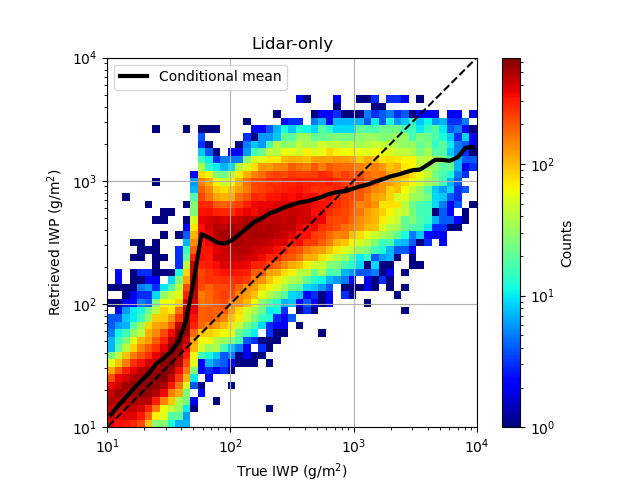
\includegraphics[width=.481\linewidth]{fig07a.rev.png}
    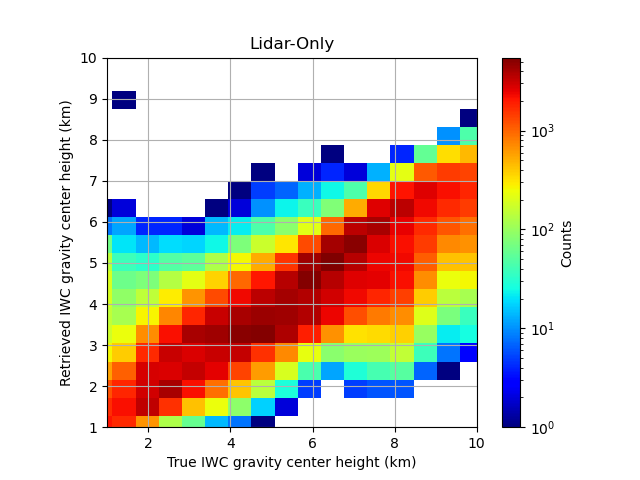
\includegraphics[width=.481\linewidth]{fig07c.rev.png}
    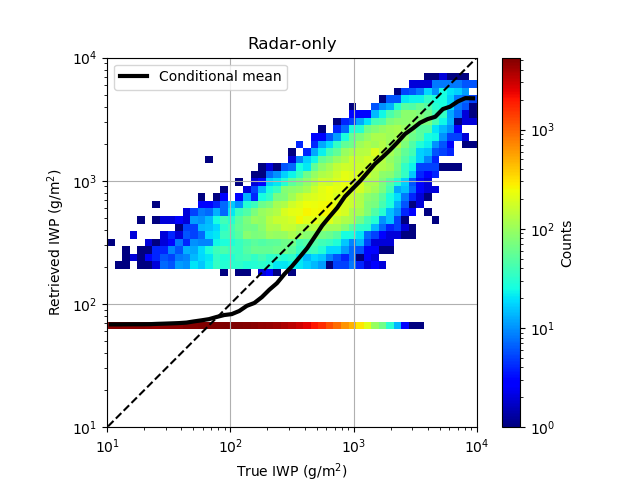
\includegraphics[width=.481\linewidth]{fig07b.rev.png}
    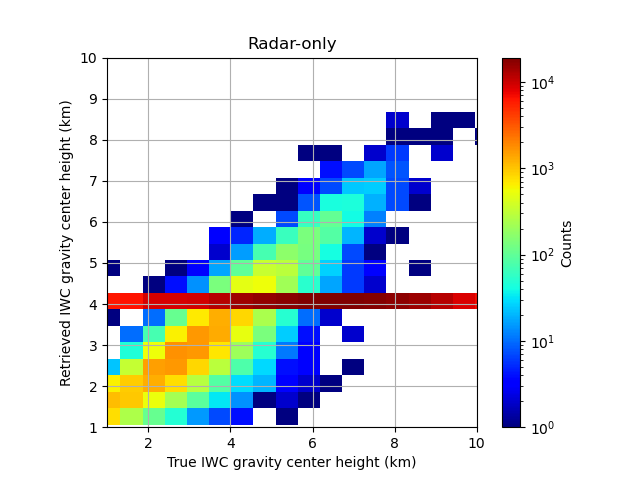
\includegraphics[width=.481\linewidth]{fig07d.rev.png}
    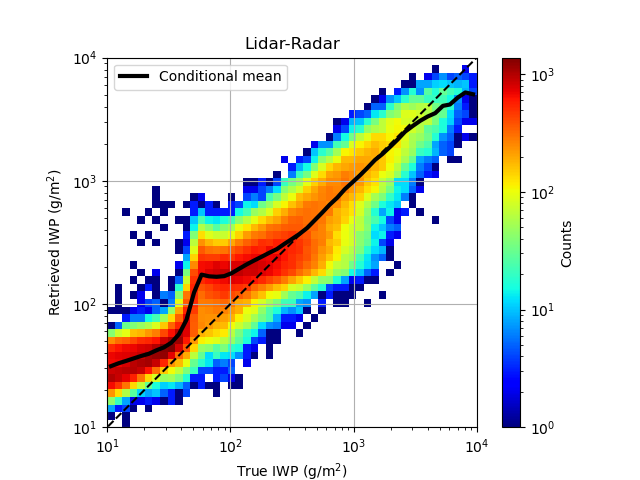
\includegraphics[width=.481\linewidth]{fig7e0.png}
    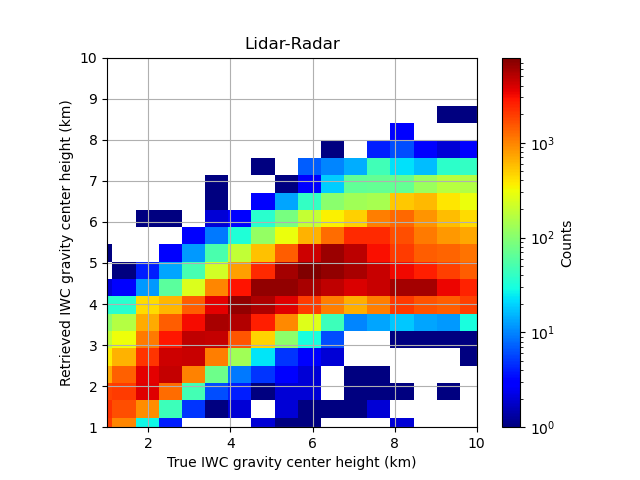
\includegraphics[width=.481\linewidth]{fig7e.png}
    \caption{Top Row: Density plots of lidar-only IWP retrievals (left), and retrieved IWC gravity centers (right) observations as a function of their true values. Middle Row: Same as in the top row but for radar-only retrievals. Bottom Row: Same as in the top row but for lidar-radar retrievals}\label{f7}
\end{figure}

\subsection{Synergistic retrievals}

The synergy of the instrument on the estimates may be investigated by simply incorporating lidar and radar observations into the retrieval process and comparing the results with the radiometer-only estimates.  Although the lidar observations are subject to attenuation, they are able to provide information about the vertical distribution of ice in clouds, mostly at the top of the clouds. The radar observations, on the other hand, are able to provide information in the bottom part of the clouds, where the lidar signal is below the noise level due to attenuation. Therefore, the combined used of lidar and radar observations is expected to provide a more complete characterization of the vertical distribution of ice in clouds and enable the derivation of more specific estimates than those derived from radiometer-only observations. It should be mentioned that, although deficiencies and potential biases in the simulated observations may distort conclusions to some degree, the forward models used in this study are state-of-the-art and are expected to enable a realistic characterization of the impact of individual instruments on the synergistic retrievals.

Shown in Figure \ref{f8} is the distribution of the synergistic IWP estimates as a function of their true values.  As apparent in the figure, the synergistic IWP estimates are more accurate than the radiometer-only estimates. At the same time, as apparent in Figure \ref{f9}, the retrieved conditional mean IWC for the 18 classes described section 2a and shown in Figure \ref{f1} are in significantly better agreement with the true IWC profiles than those derived from radiometer-only observations.  Moreover, as seen in Figure \ref{f10} the synergistic IWC gravity center estimates are in much better agreement with the true IWC gravity center than those derived from single-instrument observations.

\begin{figure}[t]
    \centering
    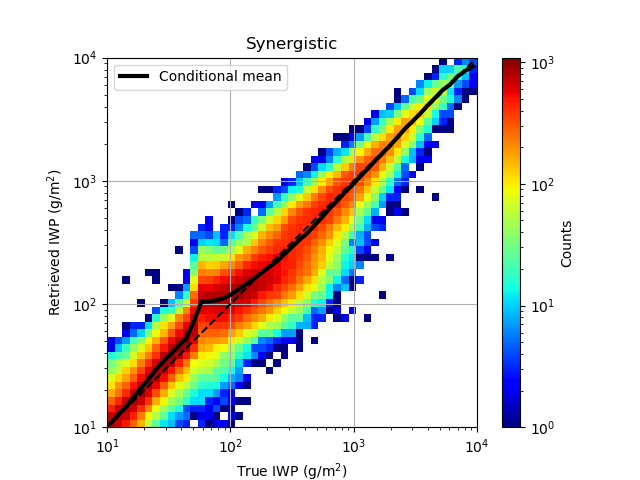
\includegraphics[width=0.75\textwidth,angle=0]{fig08.rev.png}\\
    \caption{Same as in Figure \ref{f4}, but with the lidar and radar observations incorporated in the
    retrievals.}\label{f8}
\end{figure}

\begin{figure}[t]
    \centering
    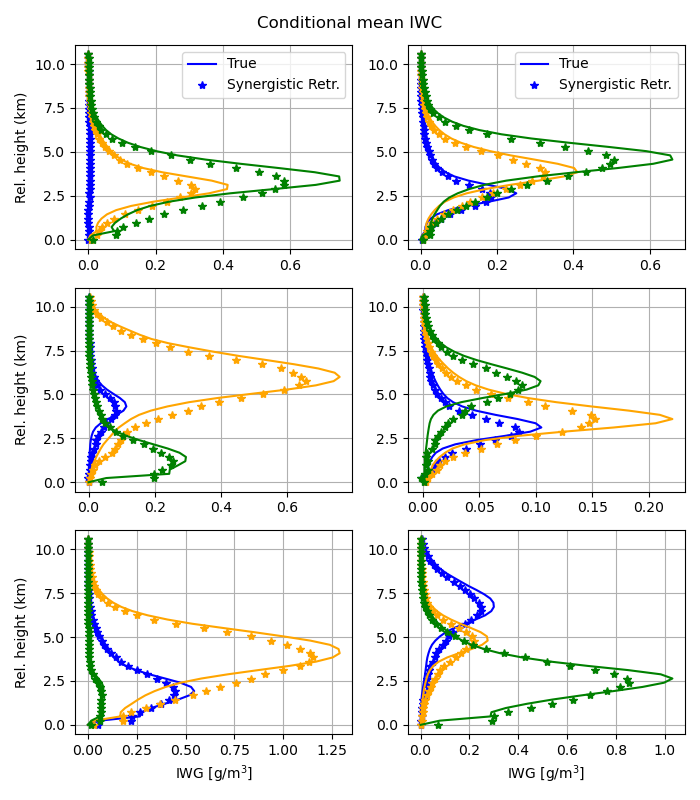
\includegraphics[width=0.75\textwidth,angle=0]{fig09.rev.png}\\
    \caption{Same as in Figure \ref{f5}, but with the lidar and radar observations incorporated in the
    retrievals.}\label{f9}
\end{figure}

While the estimates based on all instruments are significantly more accurate than those based on radiometer-only observations, it is useful to investigate how the two active instruments (lidar and radar) impact the estimates.  For conciseness, we use two statistical scores, namely, the normalized root mean square (NRMS) and the classification accuracy, to summarize the performance of the estimates.  The NRMS is defined as
\begin{equation}
NRMS=\frac {\sqrt {\frac {\sum_{i=1}^{N} (IWC_{i}-IWC_{true,i})^2} {N}}} {\sqrt {\frac {\sum_{i=1}^{N} (IWC_{true,i}-\overline{IWC})^2} {N}}} 
\end{equation}
where IWC$_{i}$ is the estimated IWC for the $i$-th sample, IWC$_{true,i}$ is the true IWC for the $i$-th sample,
$\overline{IWC}$ is the IWC mean, and $N$ is the size of the estimation dataset.  The classification
accuracy is defined as
\begin{equation}
CA=\frac {\sum_{i=1}^{N} \delta_{i}} {N}
\end{equation}
where $\delta_{i}$ is a binary variable that is equal to 1 if the estimated IWC class for the $i$-th sample is equal to the true IWC class for the $i$-th sample, and 0 otherwise. The performance summary is shown in Table \ref{t1} for several combinations of instruments. It may be observed in the table that the performance of the estimates based on all instruments is significantly better than those based on radiometer-only observations.  Furthermore, the inclusion of the lidar observations in the retrieval process has a larger impact on the retrieval performance than the inclusion of the radar
observations.  This is expected since the lidar observations are able to provide information about the top of the clouds, where the radar observations are above the noise level only occasionally. Nevertheless, the inclusion of the radar observations in the retrieval process has a notable impact on the accuracy of the IWC estimates relative to radiometer-only retrievals. 

Additional insight may be gained by examining the distribution of the retrieved of IWP and IWC gravity center as a function of their true values.  These distributions are show in Figure \ref{f11} for the lidar-radiometer and radar-radiometer retrievals.  As apparent in the figure, the inclusion of radiometer observations improves both the lidar and radar retrievals. However, neither of the two instrument combinations is able to provide estimates that are as accurate as those derived from all instruments.  Moreover, the lidar-radiometer IWP retrievals appear to be less accurate than lidar-only retrievals. This may be an artifact of statistical inversion methodology, which may make suboptimal use of correlations in the observations and improve the accuracy of the estimates for some type of profiles at the expense of others.  While other statistical inversion methodologies may be able to eliminate this artifact, given the complexity of the problem and the multiple sources of uncertainty, no better methodology is
obvious yet.


\begin{figure}[t]
    \centering
    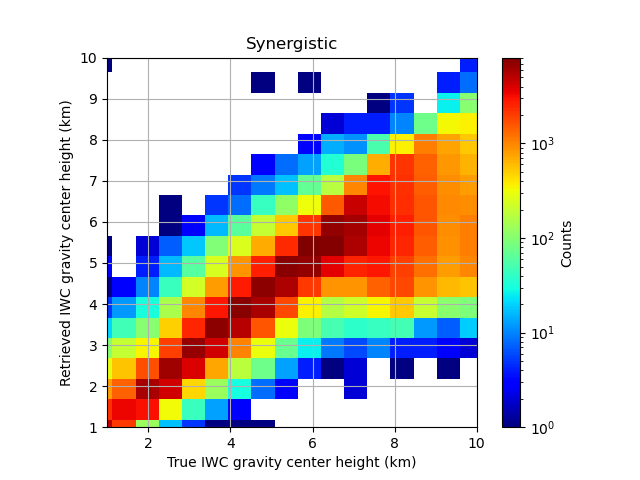
\includegraphics[width=0.75\textwidth,angle=0]{fig10.rev.png}\\
    \caption{Same as in Figure \ref{f6}, but with the lidar and radar observations incorporated in the
    retrievals.}\label{f10}
\end{figure}

\begin{figure}
    \centering
    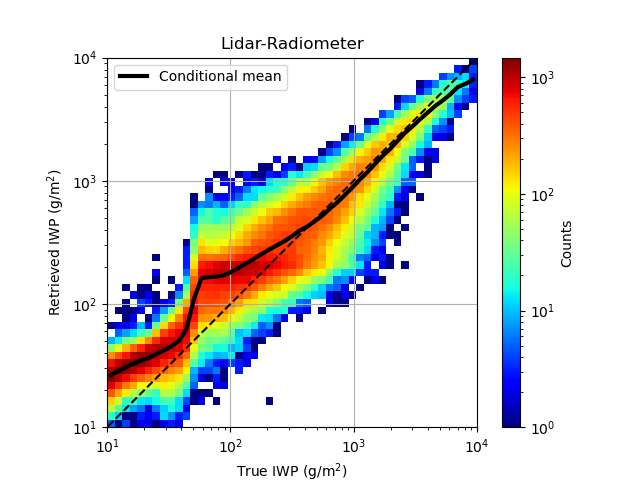
\includegraphics[width=.481\linewidth]{fig11a.rev.png}
    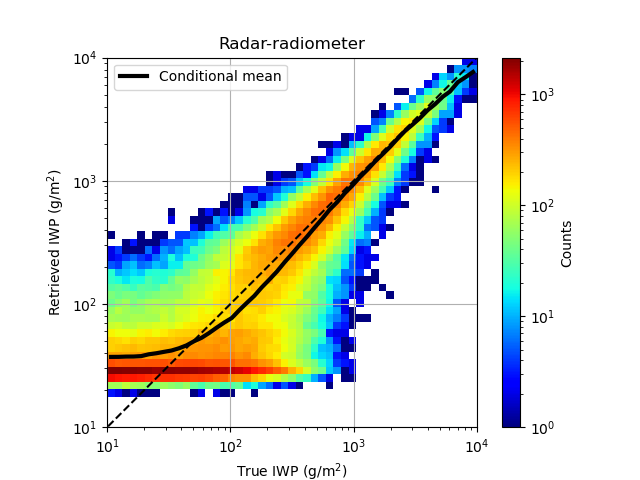
\includegraphics[width=.481\linewidth]{fig11b.rev.png}
    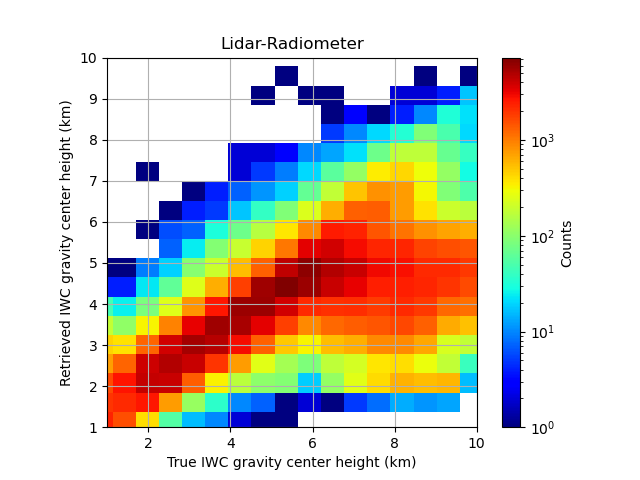
\includegraphics[width=.481\linewidth]{fig11c.rev.png}
    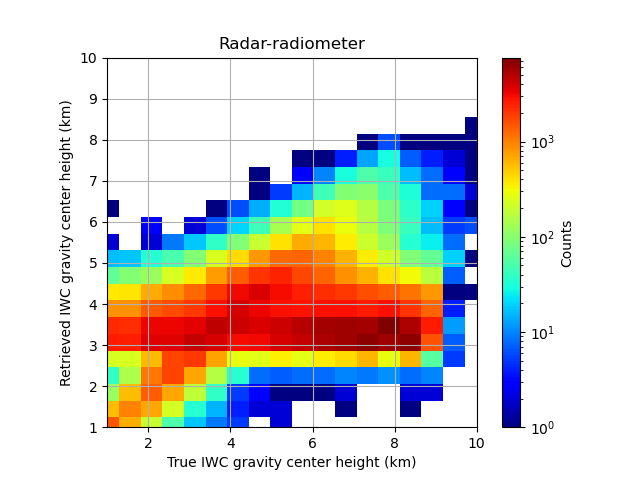
\includegraphics[width=.481\linewidth]{fig11d.rev.png}
    \caption{Top Row: Density plots of IWP retrievals from lidar-radiometer (left), and radar-radiometer (right) observations as a function
    of true IWP. Bottom Row: Same as in the top row but for IWC gravity center.}\label{f11}
\end{figure}

%Therefore, results in table
%\ref{t1} are in agreement with a qualitative analysis.  Specifically, given the 
%limited sensitivity of the Ku-band radar, the fraction of profiles with radar 
%observations above the noise level is relatively small.  On the other hand, 
%the lidar provides useful information that may be used to more accurately 
%identify the most likely vertical IWC distribution class for all profiles. 



\begin{table}[t]
\caption{Performance summary.}\label{t1}
\begin{center}
\begin{tabular}{c|ccccccc}
\hline\hline
\backslashbox{Score}{Instruments} & Lidar-& Radar- & Radiometer- & Lidar- & 
Lidar- & Radar-	& Lidar-\\
 & Only & Only & Only & Radar & Radiometer& Radiometer & Radar-Radiometer\\
\hline
% NRMS & 0.73 &  0.59  &  0.32 & 0.32 \\
NRMS & 0.84	& 0.67 & 0.64 & 0.61 &	0.56 &	0.54 &	0.48 \\
%0.73 &  0.59  &  0.32 & 0.22 \\
Class. Accurracy & 0.40	& 0.39 &	0.35 &	0.49 &	0.62& 0.53	& 0.64 \\
\hline
\end{tabular}
\end{center}
\end{table}

% text...
% 
\section{Conclusions}
In this study, we investigate the synergy of elastic backscatter lidar, Ku-band radar, and sub-millimeter-wave radiometer measurements in the retrieval of the ice from satellite observations.  The synergy is analyzed through the generation of a large dataset of IWC profile and the calculation of lidar, radar and radiometer observations using realistic models. The characteristics of the instruments (e.g. frequencies, sensitivities, etc.) are set based on the expected characteristics of instruments of the AOS mission. A hold-out validation methodology is used to assess the accuracy of the retrieved IWC profiles from various combinations of observations from the three instruments. Specifically, the IWC and associated observations is randomly divided into two datasets, one for training and the other for evaluation.  The training dataset is used to train the retrieval algorithm, while the evaluation dataset is used to assess the retrieval performance. 

To ensure the self-consistency of results and their relevance to practical applications, the dataset of IWC profiles is derived from CloudSat reflectivity observations and extended with lidar-based estimates from the 2C-ICE product. Although subject to potential biases and uncertainties due to deficiencies in the retrieval models, these profiles are deemed to be more realistic than those derived from cloud resolving model simulations. Moreover, they are roughly consistent with
the 2C-ICE CloudSat product \citep{deng2015}, while relying on assumptions and parameterizations that enable the accurate computation of backscatter lidar, Ku-band radar, and sub-millimiter-wave radiometer observations.

The retrieval of the ice water content (IWC) profiles from the computed observations is achieved in two steps.  In the first step, a class, out of 18 potential classes characterized by different  vertical distribution of IWC, is estimated from the observations. The 18 classes are predetermined based on k-Means clustering algorithm.  In the second step, the IWC profile is estimated using an Ensemble Kalman Smoother (EKS) algorithm that uses the estimated class as a priori information.

The results of the study show that the synergy of lidar, radar, and radiometer observations is significant in the retrieval of the IWC profiles.  The inclusion of the lidar observations in the retrieval process has a larger impact on the retrieval performance than the inclusion of the radar observations.  Although results are not directly comparable to those from other studies \citep{pfreundschuh2020synergistic,liu2022assessing}, given the differences between the instruments in this study relative to those from other studies, it may be concluded that they are not inconsistent with previous studies. Specifically, previous studies show some skills in radiometer-only retrievals and significant improvements in the retrieval performance when the active observations are incorporated. From this perspective, our findings are consistent with previous studies.

Further work is necessary to assess the impact of sources of uncertainties such as potential biases in the forward models, variability in the PSD intercept not captured by the current parameterization, differences in the instruments' footprint sizes, and non-uniform beam filling on the retrievals of the IWC profiles.  Other sources of uncertainties that need be considered include the potential existence of supercooled liquid water in the clouds and uncertainties in the electromagnetic scattering properties used in the in instruments' forward models. These uncertainties may be best investigated and mitigated through the use of high-quality observations from field campaigns such as The Investigation of Microphysics and Precipitation for Atlantic Coast-Threatening Snowstorms (IMPACTS) \citep{mcmurdie2022}. To achieve its objectives, which were driven by the need to improve the understanding of snowfall processes, remote sensing of snow, and the prediction of banded snow structures \citep{mcmurdie2022}, IMPACTS relied on a suite of active and passive instruments deployed via a satellite-simulating aircraft. These included multiple radars, one of them operating at Ku-band, a 532 nm elastic lidar, and a sub-millimeter-wave radiometer similar to the one considered in this study. While the objectives of IMPACTS were snowstorms, the instruments used in the campaign sampled a wide range of clouds, including high ice clouds.  The IMPACTS observations associated with high ice clouds may be used to derive IWC estimates that may be directly validating using "in-situ" measurements, as the high-altitude aircraft flew in coordination with a cloud penetrating aircraft that carried cloud and ice particle probes. These data, although not fully available yet, are expected to provide valuable information on the accuracy of the IWC retrievals from synergistic lidar, Ku-band radar and sub-millimeter-wave radiometer observations and enable the refinement of the retrieval algorithm formulated in this study. As such, they are considered a priority for future work.


%%%
% \section{First primary heading}

% \subsection{First secondary heading}

% \subsubsection{First tertiary heading}

% \paragraph{First quaternary heading}

%%%%%%%%%%%%%%%%%%%%%%%%%%%%%%%%%%%%%%%%%%%%%%%%%%%%%%%%%%%%%%%%%%%%%
% TABLES---INSERT NEAR IN-TEXT DISCUSSION
%%%%%%%%%%%%%%%%%%%%%%%%%%%%%%%%%%%%%%%%%%%%%%%%%%%%%%%%%%%%%%%%%%%%%
%%  Enter tables near where they are discussed within the document. 
%%  Please place tables before/after paragraphs, not within a paragraph.
%%
%


%%%%%%%%%%%%%%%%%%%%%%%%%%%%%%%%%%%%%%%%%%%%%%%%%%%%%%%%%%%%%%%%%%%%%
% FIGURES---INSERT NEAR IN-TEXT DISCUSSION
%%%%%%%%%%%%%%%%%%%%%%%%%%%%%%%%%%%%%%%%%%%%%%%%%%%%%%%%%%%%%%%%%%%%%
%%  Enter figures near where they are discussed within the document.
%%  Please place figures before/after paragraphs, not within a paragraph.
% %
%
%\begin{figure}[t]
%  \noindent\includegraphics[width=19pc,angle=0]{figure01.pdf}\\
%  \caption{Enter the caption for your figure here.  Repeat as
%  necessary for each of your figures. Figure from \protect\cite{Knutti2008}.}\label{f1}
%\end{figure}

\clearpage
%%%%%%%%%%%%%%%%%%%%%%%%%%%%%%%%%%%%%%%%%%%%%%%%%%%%%%%%%%%%%%%%%%%%%
% ACKNOWLEDGMENTS
%%%%%%%%%%%%%%%%%%%%%%%%%%%%%%%%%%%%%%%%%%%%%%%%%%%%%%%%%%%%%%%%%%%%%
\acknowledgments
This work was supported by the NASA Remote Sensing Theory project through Grant 80NSSC20K1729. 
The authors thank Dr. Lucia Tsaoussi (NASA Headquarters) for her support of this effort.
%  Keep acknowledgments (note correct spelling: no ``e'' between the ``g'' and
% ``m'') as brief as possible. In general, acknowledge only direct help in
%  writing or research. Financial support (e.g., grant numbers) for the work done, 
%  for an author, or for the laboratory where the work was performed must be 
%  acknowledged here rather than as footnotes to the title or to an author's name.
%  Contribution numbers (if the work has been published by the author's institution 
%  or organization) should be placed in the acknowledgments rather than as 
%  footnotes to the title or to an author's name.

%%%%%%%%%%%%%%%%%%%%%%%%%%%%%%%%%%%%%%%%%%%%%%%%%%%%%%%%%%%%%%%%%%%%%
% DATA AVAILABILITY STATEMENT
%%%%%%%%%%%%%%%%%%%%%%%%%%%%%%%%%%%%%%%%%%%%%%%%%%%%%%%%%%%%%%%%%%%%%
% 
%
\datastatement
The CloudSat data can be accessed at: https://www.cloudsat.cira.colostate.edu/.
%  The data availability statement is where authors should describe how the data underlying 
%  the findings within the article can be accessed and reused. Authors should attempt to 
%  provide unrestricted access to all data and materials underlying reported findings. 
%  If data access is restricted, authors must mention this in the statement. See
%  {http://www.ametsoc.org/PubsDataPolicy} for more info.

%%%%%%%%%%%%%%%%%%%%%%%%%%%%%%%%%%%%%%%%%%%%%%%%%%%%%%%%%%%%%%%%%%%%%
% APPENDIXES
%%%%%%%%%%%%%%%%%%%%%%%%%%%%%%%%%%%%%%%%%%%%%%%%%%%%%%%%%%%%%%%%%%%%%
%
%% If only one appendix, use

%\appendix

%% If more than one appendix, use \appendix[<letter>], e.g.,

%\appendix[A] 

%% Appendix title is necessary! For appendix title:

%\appendixtitle{Title of Appendix}

%%% Appendix section numbering (note, skip \section and begin with \subsection)
%
% \subsection{First primary heading}

% \subsubsection{First secondary heading}

% \paragraph{First tertiary heading}


%%%%%%%%%%%%%%%%%%%%%%%%%%%%%%%%%%%%%%%%%%%%%%%%%%%%%%%%%%%%%%%%%%%%%
% REFERENCES
%%%%%%%%%%%%%%%%%%%%%%%%%%%%%%%%%%%%%%%%%%%%%%%%%%%%%%%%%%%%%%%%%%%%%
% Make your BibTeX bibliography by using these commands:
\bibliographystyle{ametsocV6}
\bibliography{references}


\end{document}